\chapter{Evaluación}
\label{chap:evaluation}
\vspace{0.5cm}

%%%%%%%%%%%%%%%%%%%%%%%%%%%%%%%%%%%%%%%%%%%%%%%%%%%%%%%%%%%%%%%%%%%%%%%%%%%%%%%%
% Objetivo: Exponer los resultados objetivos del sistema                       %
%%%%%%%%%%%%%%%%%%%%%%%%%%%%%%%%%%%%%%%%%%%%%%%%%%%%%%%%%%%%%%%%%%%%%%%%%%%%%%%%

 \lettrine{E}{n} este capítulo exponen los resultados de la evaluación del sistema. Se han seleccionado tres piezas musicales conocidas para realizar las diferentes pruebas. A continuación se describen las tres piezas y las pruebas realizadas. Para realizar una prueba de carga que establezca los límites del sistema se ha añadido una última partitura suficientemente sencilla sobre la que trabajar para poder realizar estas pruebas cómodamente sin preocuparse por la calidad de los resultados.
 
 \begin{itemize}
 	\item \textbf{Menuet en Sol Mayor:} Famosa pieza de Johann S. Bach, destaca por su simpleza y es interesante para ver como funciona el programa ante compases ternarios. Se sugiere añadir una voz nueva de tesitura más grave a la presente en la pieza. (Ver Figura \ref{fig:menuet_extra_bass})
 	\item \textbf{Greensleves:} Supuestamente compuesta por Enrique VIII, esta archiconocida partitura presenta una polifonía coral a cuatro voces, ideal para comprobar las capacidades de armonización del sistema. Se sugiere eliminar secciones de alguna voz y ver cómo la completa. (Ver Figuras \ref{fig:greensleeves_harm} y \ref{fig:greensleeves_measure})
 	\item \textbf{Joy to the World:} Conocido villancico de Georg F. Händel, sería interesante escuchar una reinterpretación de la voz más grave para la pieza, ya sea completando secciones o bien añadiendo una voz de bajo (Ver Figura \ref{fig:joy_harm}).
    \item \textbf{Twinkle Twinkle Little Star:} Esta sencilla pieza popular es adecuada para realizar, además de pruebas similares a otras piezas, pruebas de carga para comprobar como crecen los tiempos de búsqueda y hallar los límites de la herramienta (Ver Figuras \ref{fig:twinkle_harm} y \ref{fig:twinkle_measure}).
 \end{itemize}
 
 Para la evaluación se han realizado armonizaciones de todas las piezas y se han medido los tiempos y la calidad de las mismas, además se han realizado pruebas de completado de un compás en cada pieza junto con la inclusión de una nueva voz, también se han medido calidad y tiempo. Por último, con la última partitura se han realizado pruebas para comprobar hasta donde funciona bien en cuestión temporal, para ello se ha ido vaciando porcentualmente una de las voces para ser completada y después se han ido añadiendo diferentes voces. Las figuras de esta sección sirven para ilustrar algunos resultados obtenidos, se puede comparar con las partituras originales presentes en el Apéndice \ref{chap:scores} Partituras.
 
 Nótese que debido al carácter no-determinista de \textit{Answer Set Programming} y a los tiempos de entrada y salida estos tiempos sirven para dar una idea aproximada de los tiempos de funcionamiento de la herramienta. Para suavizar los valores dispares se ha ejecutado cada medida 100 veces, se ha restado el tiempo de usuario y se ha calculado el tiempo promedio. 


\begin{figure}
	\centering
	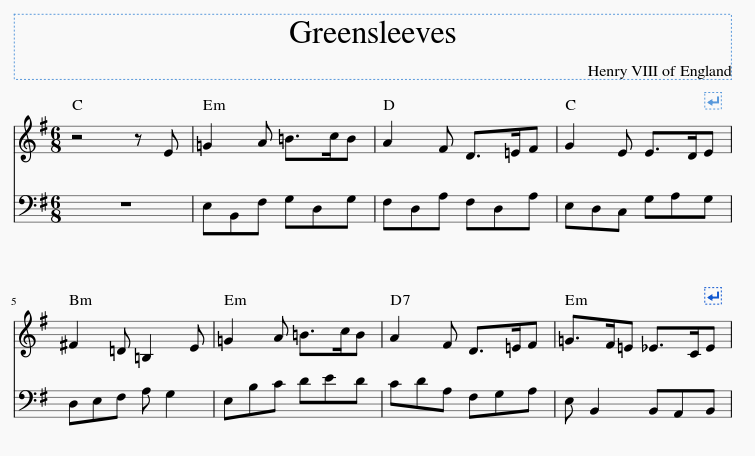
\includegraphics[width=0.8\linewidth]{imagenes/evaluation/greensleeves_harm.png}
	\caption{Comienzo de Greensleeves armonizado}
	\label{fig:greensleeves_harm}
\end{figure}

\begin{figure}
   	\centering
   	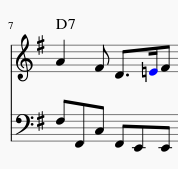
\includegraphics[width=0.2\linewidth,valign=c]{imagenes/evaluation/greensleeves_measure.png}
   	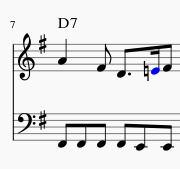
\includegraphics[width=0.2\linewidth,valign=c]{imagenes/evaluation/greensleeves_measure_melodious.png}
   	\caption{Compás de Greensleeves completado sin y con preferencias melódicas activadas}
   	\label{fig:greensleeves_measure}
\end{figure}



\begin{figure}
    	\centering
    	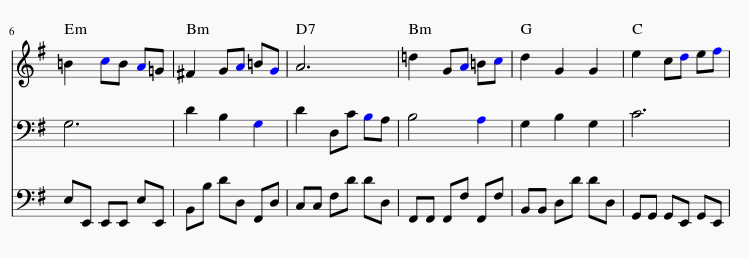
\includegraphics[width=0.9\linewidth]{imagenes/evaluation/menuet_extra_bass.png}
    	\caption{Menuet con una voz de Bajo adicional (sin preferencias melódicas)}
    	\label{fig:menuet_extra_bass}
\end{figure}

\begin{figure}
    	\centering
    	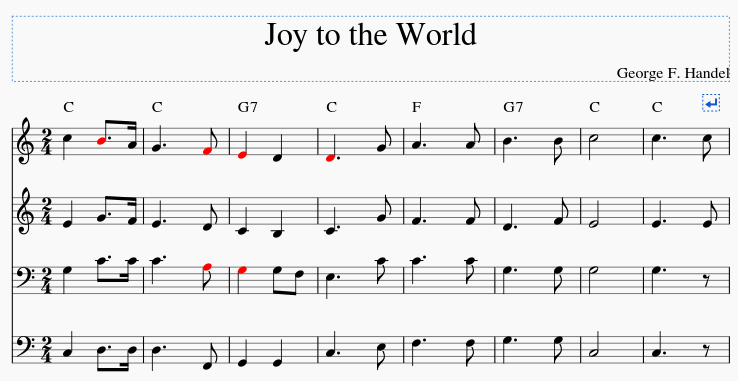
\includegraphics[width=0.8\linewidth]{imagenes/evaluation/joy_harm.png}
    	\caption{Comienzo de Joy to the World armonizado}
    	\label{fig:joy_harm}
\end{figure}



\begin{center}
	\begin{tabular}{ | l | c | c | c | }
		\hline
		Pieza 			& T. Armonización 	& T. Compás & T. Nueva voz \\ \hline \hline
		Greensleeves 	& 1.016s 			& 1.926s	& 4m 49.032s \\ \hline
		Menuet 			& 0.631s 			& 0.726s 	& 3m 50.376s \\ \hline
		Joy to the World& 2.381s 			& 3.813s	& 7m 17.115s \\ \hline
		Twinkle Twinkle & 0.685s 			& 0.716s 	& 2m 31.299s \\ \hline
	\end{tabular}
\end{center}

Cuantitativamente, los resultados del sistema son los esperados. Los tiempos de armonización de partituras son excepcionalmente buenos y los de completado de secciones obtienen resultados muy interesantes ya que para un compás vacío se puede observar un escaso segundo de diferencia. No obstante, se ha podido comprobar que el crecimiento de tiempo necesario para completar una partitura no es lineal, ya que al haber cada vez más figuras que completar, surgen más posibilidades combinatorias.

Esto queda reflejado en el tiempo necesario para añadir una nueva voz a la partitura, que crece hasta el orden de los minutos para una voz. No resulta problemático, ya que teniendo en cuenta la cantidad de posibilidades sigue siendo un orden de tiempo aceptable para hallar el mejor resultado posible, si tenemos en cuenta que podemos especificar un timeout, podríamos obtener un resultado aceptable (por ejemplo una voz nueva con una ratio de errores por nota de alrededor del 10\%) en prácticamente la mitad de tiempo.

Cualitativamente, los resultados de armonización son adecuados y el completado de secciones o la inclusión de nuevas voces ofrece soluciones interesantes y correctas armónicamente. En algunos casos, por culpa del módulo se dalida, se producen errores visuales al asignar la clave de forma equivocada (Ver Figura \ref{fig:joy_harm_err}), pero este error es subsanable en el editor de partituras y no presenta ningún fallo real en la armonización ni completado. 

\begin{figure}
    	\centering
    	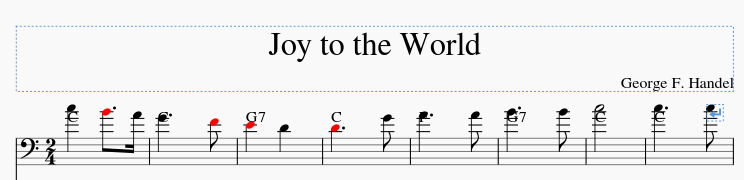
\includegraphics[width=0.9\linewidth]{imagenes/evaluation/joy_harm_err.png}
    	\caption{La salida de Joy to the World produce un error de clave en la voz de la Soprano}
    	\label{fig:joy_harm_err}
\end{figure}

Las pruebas de carga sobre ``Twinkle Twinkle Little Star'' se han realizado primero vaciando progresivamente una de las voces. La pieza cuenta con 24 compases, se han vaciado 4 compases en cada iteración, aunque no se ha vaciado del todo la voz ya que eso corresponde al siguiente punto. Por último se han ido añadiendo voces, una voz de una tesitura diferente en cada iteración.
\begin{center}
	\begin{tabular}{ | l | r | }
		\hline
		Prueba & Tiempo \\ \hline
		4 compases  & 1.481s \\ \hline
		8 compases 	& 2.394s \\ \hline
		12 compases	& 3.978s \\ \hline
		16 compases & 3.982s \\ \hline
		20 compases & 5.966s \\ \hline
		1 voz & 2m 31.299s \\ \hline
		2 voces & 25m 17.298s  \\ \hline
	\end{tabular}
\end{center}

\begin{figure}
     	\centering
     	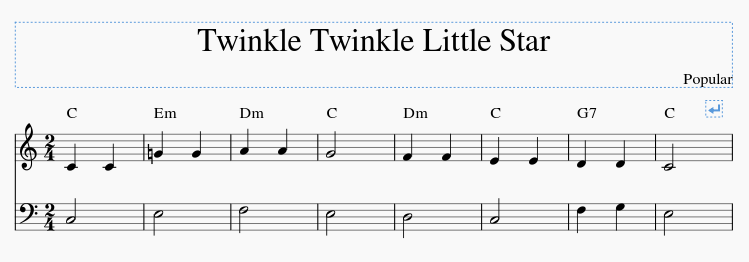
\includegraphics[width=0.8\linewidth]{imagenes/evaluation/twinkle_harm.png}
     	\caption{Comienzo de Twinkle Twinkle Little Star armonizado}
     	\label{fig:twinkle_harm}
\end{figure}

\begin{figure}
   	\centering
   	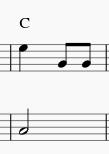
\includegraphics[width=0.2\linewidth,valign=c]{imagenes/evaluation/twinkle_measure.png}
   	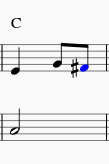
\includegraphics[width=0.2\linewidth,valign=c]{imagenes/evaluation/twinkle_measure_melodious.png}
   	\caption{Compás de Twinkle Twinkle Little Star completado sin y con preferencias melódicas activadas}
   	\label{fig:twinkle_measure}
\end{figure}

No se realizaron ejecuciones con más de dos voces adicionales ya que el tiempo de ejecución ya se dispara a las decenas de minutos y no se consideró relevante, se puede establecer el límite del funcionamiento usable en dos voces si se interrumpe la ejecución o en una voz completa. Puede resultar curioso que una pieza casi vacía (como en el ejemplo de 20 compases vacíos) siga en el orden de segundos mientras que una voz nueva se va a los minutos. La explicación de esto radica en las figuras completables contra las nuevas voces. Las figuras completables cuentan con un patrón rítmico determinado al que se ajustan las notas, reduciendo drásticamente la cantidad de notas que hay que calcular para la solución. En una nueva voz no existe este patronaje rítmico, las figuras son siempre la figura base con la que se ha armonizado y subdividido internamente toda la pieza, resultando siempre en tener que calcular el máximo de notas en cada voz. Para solucionar esto se pueden incluir voces nuevas en la partitura directamente en el editor, especificando los patrones rítmicos, en lugar de a través de la línea de comandos.

\section{Comparativa}
El presente proyecto es un sistema relativamente único en cuanto a qué hace y cómo lo hace. La única herramienta comparable sería el software ANTON \cite{anton-composing} ya que ambos tienen su fundamento en \textit{Answer Set Programming}, pueden trabajar sobre partituras ya creadas y funcionan mediante módulos destinados a las diferentes partes del proceso de composición. La gran diferencia radica en que ANTON es un sistema mucho más complejo que el presente, permitiendo componer no solo armónica sino también melódicamente y, además, ANTON contempla la creación de patrones rítmicos. Por otra parte, el proyecto aquí creado ahonda más en la armonía que ANTON, permitiendo simplemente armonizar una pieza completa y completar partituras de cualquier número de voces y estilos, mientras que ANTON se limita a la composición de piezas de dos voces en un estilo renacentista concreto.

Ya que ANTON trabaja siempre con dos voces resulta algo complejo comparar tiempos de ejecución, pero las pruebas realizadas al sistema para duetos de 32 compases completamente nuevos daban resultados en el orden de los minutos. El sistema actual presenta un rendimiento similar a la hora de crear una segunda voz para convertir una pieza monofónica en un dueto, pero al no contemplar ritmo y necesitar la primera voz para componerla, puede verse la inferioridad del sistema frente a ANTON.

  \section{Problemas conocidos}
  \label{sec:known_issues}
  Las diferentes pruebas han revelado ciertos problemas que se producen si no siempre, sí lo hacen con una frecuencia relativamente alta y que por diseño de la herramienta no han sido atacados. En la sección de \ref{sec:future_work} Trabajo Futuro en el capítulo \ref{chap:conclusiones} Conclusión se detalla cuales de ellos se pretenden arreglar a corto o medio plazo.
  
  \begin{itemize}
  		\item \textbf{Tresillos:} Los tresillos, dosillos y otras figuras irregulares no funcionan correctamente en la herramienta y han de ser editados en la partitura antes de procesarla. Esto se debe a que no es posible realizar una subdivisión directa a la nota base de la partitura de este tipo de figuras.
  		\item \textbf{Clave:} Algunas voces aparecen en la salida con la clave mal identificada, produciendo un resultado poco legible. Esto es fácilmente solucionable cambiando la clave de la voz correspondiente en el archivo de salida, ya que pese a todo, esto es un fallo meramente visual y no afecta a los valores de las notas de la voz.
  		\item \textbf{Nombres de Tesituras:} Si bien los nombres de las voces corales no varían sustancialmente, los nombres de los instrumentos sí lo hacen, por esto el \textit{locale} de la herramienta usada para la edición de partituras puede producir incompatibilidades a la hora de restringir el rango de voces, por ejemplo, una partitura para escrita para Violonchelo en un sistema en castellano marcará esa voz como \texttt{voice\_type(x, violonchelo)} mientras que un sistema en inglés producirá  \texttt{voice\_type(x, violoncello)}. Para solucionarlo se ruega editar el fichero \texttt{voice\_types.lp} en la carpeta \texttt{asp/include} para que los límites de cada instrumento se correspondan con el locale del sistema.
  		\item \textbf{Falsos positivos:} Debido a que en algunas figuras como los conjuntos de corcheas o semicorcheas consecutivas no se puede identificar los subtiempos débiles y fuertes que no dependen del compás si no de la propia figura junto con algunas dificultades a la hora de identificar los tiempos débiles y fuertes de un compás con las notas subdivididas y después transformarlo a otro tipo de compás, es probable que algunas notas marcadas como error en la partitura no lo sean realmente.
  \end{itemize}
  

